\documentclass{article}
\usepackage{graphicx} % Required for inserting images
\usepackage{array}
\usepackage{a4wide}
\usepackage{cryptocode}

\begin{document}
\section{current sec model to transcribe ADEM + AMAC to a more symmetric style}
\subsection{used primitives}
\begin{itemize}
    \item ADEM: input tag, key en message lead to a cythertext. It should be improbable distinguish the cythertexts of two messages. (adversary may choose two cyhtertexts and has to guess which one of the two is encrypted)
    
    \item AMAC: input tag, key en message lead to a cythertext. It should be improbable to make a forgery (a pair (key, tag, message, cythertext) that verifies without begin generated by calling Omac(key, tag, message) first )
\end{itemize}

\subsection{goal}
message m is encrypted using a tag that cannot repeat and two keys to generate a cythertext concisting of two parts. First part is Cdem which is the message encrypted with the nonce and the first key while the second part is Cmac that is the mac computed over Cdem, the tag and the second key.

\subsection{Sec model}
the security is purely based on the games for the AMAC and ADEM that are visible below.\\
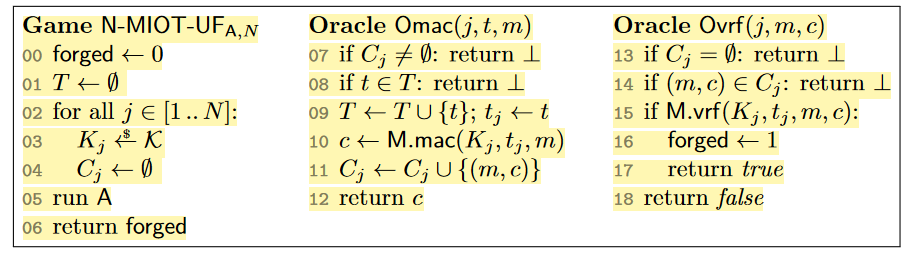
\includegraphics[scale = 0.5]{gebrabbel images/game mac.png}\\
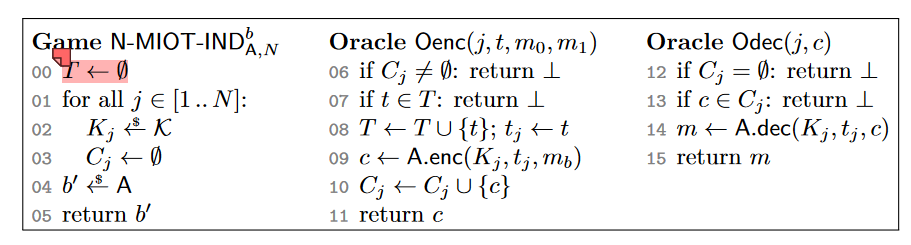
\includegraphics[scale = 0.5]{gebrabbel images/game adem.png}\\
with 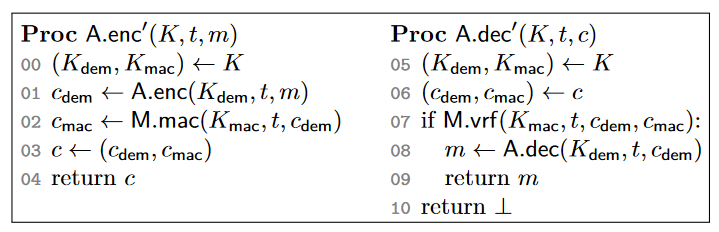
\includegraphics[scale = 0.5]{gebrabbel images/adem amac.png}\\


\newpage
\section{needed sec model to transcribe ADEM + AMAC to a more symmetric style}
for now we only look at the nonce based options as the pkc paper does that too.
\subsection{used primitives}
\begin{itemize}
    \item ADEM: input nonce, key en message lead to a cythertext which should be improbable to distinguishen from RO (adversary has to guess if he is talking to RO or ADEM)
    
    \item AMAC: input nonce, key en message lead to a tag that should be improbable to distinguishable from random oracle (adversary has to guess if he is talking to RO or AMAC)
\end{itemize}

\subsection{goal}
message m is encrypted and protected against active attacks because it is authenticated with tag T.

\subsection{Sec model}
We define the following sec games for the AMAC, the ADEM and the ADEM+AMAC (names will prob be improved later):
\begin{pchstack}[center]
\pseudocode{
    b \sample \bin 
}
\end{pchstack}

\begin{table}[h!]
\centering
\begin{tabular}{|m{4cm}  |m{6cm} |}
\hline
\textbf{Game} AMAC$^b_{A,N}$                & \textbf{Oracle} Omac(j,n,m)              \\
$used_n \leftarrow \emptyset$               & if T$_j$ $\neq \emptyset$: return $\bot$    \\
for j $\in [1..N]:$                         & if n $\in used_n$: return $\bot$               \\
\hspace{0.5cm} K$_j \leftarrow^\$ K$        & $used_n \leftarrow used_n \cup \{n\}$ \\
\hspace{0.5cm} T$_j \leftarrow \emptyset$   & n$_j \leftarrow n$  \\
b' $\leftarrow^\$ A$                        & if b=0: t $\leftarrow$ M.mac(K$_j$,n$_j$,m)     \\
return b'                                   & if b=1: t $\leftarrow$ RO.mac(K$_j$,n$_j$,m)  \\
                                            & T$_j\leftarrow$ T$_j \cup\{t\}$           \\
                                            & return t                                        \\
\hline
\end{tabular}
\caption{AMAC game}
\end{table}

\begin{table}[h!]
\centering
\begin{tabular}{|m{4cm} |m{6cm} |}
\hline
\textbf{Game} ADEM$^b_{A,N}$                & \textbf{Oracle} Oenc(j,n,m)              \\
$used_n \leftarrow \emptyset$               & if C$_j$ $\neq \emptyset$: return $\bot$    \\
for j $\in [1..N]:$                         & if n $\in used_n$: return $\bot$               \\
\hspace{0.5cm} K$_j \leftarrow^\$ K$        & $used_n \leftarrow used_n \cup \{n\}$ \\
\hspace{0.5cm} T$_j \leftarrow \emptyset$   & if b=0: c $\leftarrow$ E.enc(K$_j$,n,m)     \\
b' $\leftarrow^\$ A$                        & if b=1: c $\leftarrow$ RO.enc(K$_j$,n,m)  \\
return b'                                   & C$_j\leftarrow$ C$_j \cup\{c\}$           \\
                                            & return c                               \\
\hline
\end{tabular}
\caption{ADEM game}
\end{table}

\begin{table}[h!]
\centering
\begin{tabular}{|m{4cm}  |m{5cm}| m{5cm} |}
\hline
\textbf{Game} ADEM$^b_{A,N}$                & \textbf{Oracle} Oenc(j,n,m)                           & \textbf{Oracle} Odec(j,n,c)\\
$used_n \leftarrow \emptyset$               & if C$_j$ $\neq \emptyset$: return $\bot$              & if (c,n) $\in$ C$_j$: return $\bot$\\
for j $\in [1..N]:$                         & if n $\in used_n$: return $\bot$                      & if b = 0:\\
\hspace{0.5cm} K$_j \leftarrow^\$ K$        & $used_n \leftarrow used_n \cup \{n\}$                 & \hspace{0.5cm} m $\leftarrow$A.dec'(K$_j$,n,c)\\
\hspace{0.5cm} T$_j \leftarrow \emptyset$   & n$_j \leftarrow n$                                    & \hspace{0.5cm} return m\\
b' $\leftarrow^\$ A$                        & if b=0:                                               & if b = 1: \\
return b'                                   & \hspace{0.5cm}c $\leftarrow$ E.enc'(K$_j$,n$_j$,m)     & \hspace{0.5cm} m $\leftarrow$RO.dec'(K$_j$,n,c)\\
                                            & if b=1:
                                                & \hspace{0.5cm} return m\\
                                            & \hspace{0.5cm} c $\leftarrow$ RO.enc'(K$_j$,n$_j$,m)    & \\
                                            & C$_j\leftarrow$ C$_j \cup\{(c,n)\}$                   & \\
                                            & return c                                            & \\
\hline
\end{tabular}
\caption{ADEM + AMAC game}
\end{table}
\newpage
where E.enc, E.dec, M.mac , RO.enc, RO.dec and RO.mac are inherited from the underlying primitives and E.enc', E.dec', RO.enc' and RO.dec' will be defined later here defined.

\newpage
\section{burning questions}
\begin{itemize}
   \item 
   
\end{itemize}
\newpage
\section{current todo's}
\begin{itemize}
    \item de games opnieuw formazilen naar de nieuwe vondsten
    \item dit naar git verplaatsen
    \item crypto.bib kijken
\end{itemize}
\newpage
\section{main idea}
The PKC paper ends with a ADEM + AMAC construction as "solution". The original paper from ENC -> MAC has been revised, so this should prob be revised as well. In general its nice to write down thing in a more "sym crypto" style as we use symmetric primitives. It would probably also be nice to revise it more in general and see what other ways there are to reach the endgoal expected in the PKC paper.
\end{document}